\documentclass[10pt]{article}

% Packages with options
\usepackage[english]{babel}
\usepackage[mathscr]{euscript}
\usepackage[margin=1in]{geometry} 
\usepackage[utf8]{inputenc}
\usepackage[small]{titlesec}

% Primary Packages
\usepackage{adjustbox, amsbsy, amsmath, amssymb, amsthm, bm, commath, chngcntr, dsfont, econometrics, fancyhdr, gensymb, graphicx, IEEEtrantools, longtable, marginnote, mathrsfs, mathtools, mdframed, natbib, parskip, pgf, setspace, subfigure, tabularx, textcomp, tikz}

% Hyperref Setup
\usepackage[pdfauthor={Manu Navjeevan},
			bookmarks=false,%
			pdftitle={Econ 425 Week 7},%
			pdftoolbar=false,%
			pdfmenubar=true]{hyperref} %hyperref needs to be last

% Rest of the setup is in the "Manu" package
\usepackage{manu}

%%%%%%%%%%%%%%%%%%%%%%%%%%%%%%%%%%%%%%%%%%%%%

\title{Econ 425 Week 7}%Title
\author{Manu Navjeevan}
\date{\today}

\begin{document}
\maketitle

\section{Neural Net Review}%
\label{sec:review}

As we went over last time, a neural network consists of nodes and edges, arranged into layers.
\begin{figure}[htpb]
	\centering
	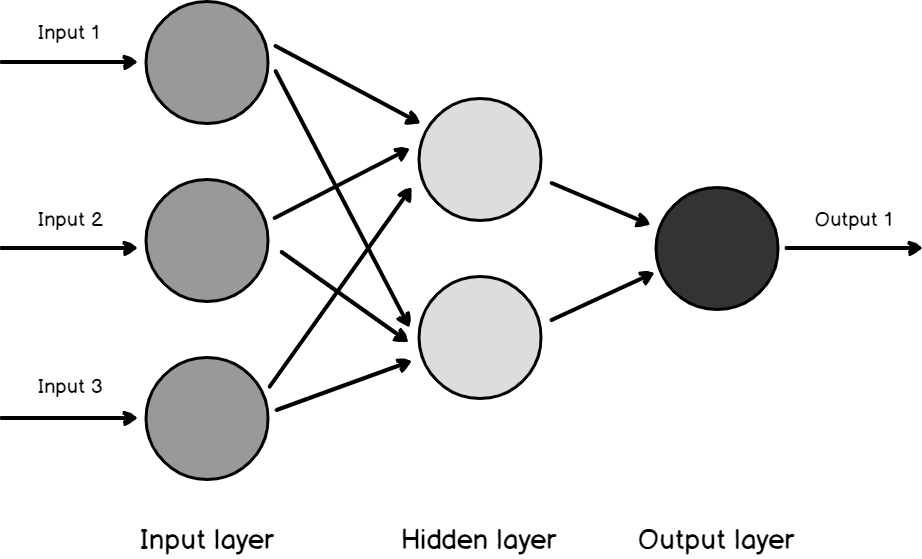
\includegraphics[width=0.8\linewidth]{neural-three.png}
	\caption{A simple neural network}%
	\label{fig:neural-three}
\end{figure}

Each neuron takes some inputs (the outputs of the neurons that are pointing to it), \(a_1,\dots,a_p\) and outputs a vector of the form:
\[
	\pi\left(\underbrace{\beta_0}_{\text{Bias Term}} + \beta_1 a_1,\dots,\beta_p a_p\right)
.\] 
where \(\pi(\cdot)\) is some pre-specified activation function. The bias term  \(\beta_0\) and each of the weights  \(\beta_1,\dots,\beta_p\) are parameters that we'd like to ``learn" using our data.

Specifically, we would like to ``learn" the parameters that minimize some cost function of our output. An example of this would be to choose the parameters that minimize the mean squared error on our training data:
\[
	MSE\left(\cdot\right) = \frac{1}{n}\sum_{i=1}^n \left(\widehat{y}_i - y_i\right)^2 
.\] 

In order to do this minimization, we essentially need to do a gradient descent on our model parameters. However, computing this gradient is not straightforward. This brings us to back propogation, which is a way of computing the gradient that takes advantage of the feed-forward nature of the neural network.  

\section{Back Propogation}%

To begin with, consider a very simple neural network. 
\begin{figure}[htpb]
	\centering
	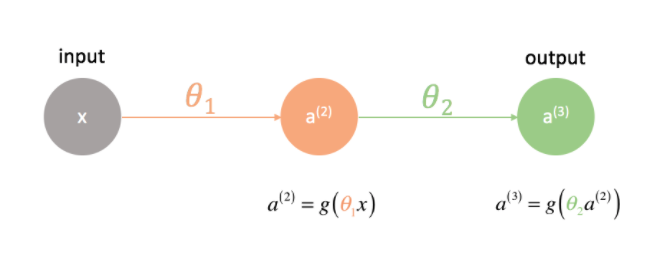
\includegraphics[width=0.8\linewidth]{simple_nn.png}
	\caption{A very simple neural net}%
	\label{fig:simple_nn}
\end{figure}

The output can be written as \(\widehat{y}_i = g\left(\theta_2\cdot g(\theta_1\cdot x_i)\right)\). My cost function is the MSE:
 \begin{align*}
	 \calC\left(\theta_1, \theta_2\right) &= \sum_{i=1}^n \left(\widehat{y}_i - y_i\right)^2 \\
										  &= \sum_{i=1}^n \left( g\left(\theta_2\cdot g(\theta_1\cdot x_i)\right)- y_i\right)^2
 \end{align*} 
I would like to compute the gradient with respect to \(\theta_1\) and  \(\theta_2\). Since this is fairly simple in this setting we do it by hand and then examine the results to gain some intuition for back propogation:
\begin{align*}
	\frac{\partial \calC}{\partial \theta_2} &= 2\sum_{i=1}^n \left(\left( g\left(\theta_2\cdot g(\theta_1\cdot x_i)\right)- y_i\right)\right)g'\left( \theta_2\cdot g(\theta_1\cdot x_i)\right)\cdot g\left(\theta_1\cdot x_i\right) \\
	\frac{\partial \calC}{\partial \theta_1} &= 2\sum_{i=1}^n \left(\left( g\left(\theta_2\cdot g(\theta_1\cdot x_i)\right)- y_i\right)\right)g'\left( \theta_2\cdot g(\theta_1\cdot x_i)\right)\cdot g'\left(\theta_1\cdot x_i\right)x_i 
\end{align*}
Comparing the partial derivatives with respect to \(\theta_2\) and  \(\theta_1\) note that the partial derivative with respect to  \(\theta_1\) can be computed iteratively. 
\begin{enumerate}
	\item First compute the derivative of the activation function in the last layer: \(g'\left(\theta_2\cdot g\left(\theta_1\cdot x_1\right)\right)\). Use these to evaluate the derivative with respect to \(\theta_2\).
	\item Compute the derivative with respect to the activation function in the first layer: \(g'\left(\theta_1 \cdot x_2\right)\). Multiply these with the derivative with the with respect to the activation function in the last layer from the first step and use the resulting product to compute the derivative with respect to \(\theta_1\).
\end{enumerate}
This provides the intuition for how back-propogation works to compute the total derivative with respect to all the weight/bias terms. To compute the total derivative we will start at the output layer, compute the derivatives of the activation function with respect to our parameters at this layer, and use these derivatives to calculate the derivative of the cost function with respect to the parameters in the last layer. To compute the derivative of the cost function with respect to parameters in the next layer back we will multiple these activation function derivatives from the final layer with the derivatives of the activation function from the next layer back layer. We then move to the second to last layer, calculate the derivatives of the activation function at each neuron and multiply these with the derivatives in the prior two layers and so on until we have the derivative with respect to every parameter.

Some notes:
\begin{itemize}
	\item Note that the first term inside the summand in each of these derivatives is \(\left(g\left(\theta_2\cdot g(\theta_1\cdot x_i)\right)-y_i\right)\). This means that observations for which our neural network prediction is far from the actual value will have a larger influence on our gradient, as we will try to correct for this and ``fix" the loss function.
	\item In the very toy example we have drawn up here we are dealing with a (trivially) ``fully connected" neural network. In practice, the multiplications at each step will depend on which nodes are connected to which. 
\end{itemize}
\begin{figure}[htpb]
	\centering
	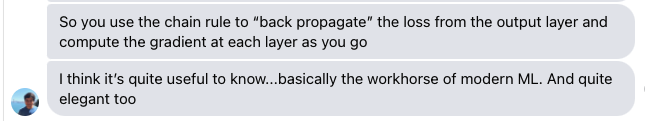
\includegraphics[width=0.8\linewidth]{shouvik.png}
	\caption{Some thoughts from my college friend Shouvik, who is working in ML.}%
	\label{fig:shouvik}
\end{figure}

\section{Overall Process}%
\label{sec:overall}

Finally, we combine our knowledge of the prediction process to come up with a unified process for ``learning" the neural net:
\begin{enumerate}
	\item Initialize a neural network with some structure (specify activation functions, layers, nodes, edges, etc.)
	\item Start with an initial guess for your parameter values (bias terms and weights at each node)
	\item Given your guessed parameter values, ``forward propogate" your inputs through your neural network to get your predicted values
	\item Given your predicted values ``backward propogate" to compute the gradient of the cost function with respect to each parameter
	\item Adjust your guess by moving in the direction of the negative gradient
	\item Repeat steps 3-5 until you reach converge to a minimum
	\item Try a few different starting guesses to make sure you have a global minimum
 \end{enumerate}



\end{document}

